\documentclass[10pt,a4paper]{article}
\usepackage[utf8]{inputenc} 
\usepackage[spanish]{babel}
\usepackage{a4wide}
\usepackage{caratula}

\begin{document}

\titulo{Trabajo Práctico}
\subtitulo{SLS: Un simple lenguaje de scripting}

\fecha{\today}

\materia{Teoría de Lenguajes}
\grupo{Los Libres de Contexto}

\integrante{Apellido, Nombre2}{002/01}{email2@dominio.com}
\integrante{Bonomi, Cyntia}{134/03}{cyntiab83@gmail.com}
\integrante{Izcovich, Sabrina}{550/11}{sizcovich@gmail.com}

\maketitle

\tableofcontents

\newpage
\section{Introducción}

\section{Gramática}
Expresiones regulares de los tokens y transformaciones\\
Tipo de Gramática definida \\


PROGRAM $\rightarrow$ LIST\_SENTENCIES \\

LIST\_SENTENCIES $\rightarrow$ SENTENCE $|$ SENTENCE LIST\_SENTENCIES\\

SENTENCE $\rightarrow$ E; $|$ WHILE $|$ IF\_ELSE $|$ CONDITIONAL $|$ FOR $|$ DO\_WHILE $|$ COMMENT \\

WHILE $\rightarrow$ while (CONDITION) SENTENCE $|$ while (CONDITION) {LIST\_SENTENCIES} \\

IF\_ELSE $\rightarrow$ IF else SENTENCE $|$ IF else {LIST\_SENTENCIES} \\

IF $\rightarrow$ if (CONDITION) SENTENCE $|$ if (CONDITION) {LIST\_SENTENCIES} \\

CONDITIONAL $\rightarrow$ (CONDITION) ? SENTENCE : SENTENCE \\

FOR $\rightarrow$ for(ASIGNACION ;CONDITION; AVANZAR) SENTENCE $|$ (ASIGNACION ;CONDITION; AVANZAR) {LIST\_SENTENCIES} \\

ASIGNACION $\rightarrow$ $\lambda$ $|$ var = EXPRESSION $|$ var[NUM] = EXPRESSION $|$ var[NUM] = EXPRESSION\\

AVANZAR $\rightarrow$ var++ $|$ var$--$ $|$ var -= NUM $|$ var += NUM $|$ $\lambda$ \\

DO\_WHILE $\rightarrow$ do LIST\_SENTENCIES while (CONDITION) \\

CONDITION $\rightarrow$ LOGICAL\_CONDITION $|$ CONDITION\_AND $|$ CONDITION\_OR \\

CONDITION\_AND $\rightarrow$ LOGICAL\_CONDITION AND LOGICAL\_CONDITION \\

CONDITION\_OR $\rightarrow$ LOGICAL\_CONDITION OR LOGICAL\_CONDITION \\

LOGICAL\_CONDITION $\rightarrow$ E $>$ E $|$ E $<$ E $|$ E == E $|$ E != E \\

E $\rightarrow$ ASIGNACION $|$ EXPRESSION \\

VALUE $\rightarrow$ string $|$ bool $|$ var $|$ NUM $|$FUNCION $|$ var[NUM] $|$ [LIST\_VALUES] $|$ LIST\_REGISTERS\\

LIST\_REGISTERS $\rightarrow$ REGISTER $|$ REGISTER , LIST\_REGISTERS\\

REGISTER $\rightarrow$ cadena:VALUE \\

LIST\_VALUES $\rightarrow$ VALUE $|$ VALUE , LIST\_VALUES \\

EXPRESSION $\rightarrow$  ARITHMETIC\_EXPRESSION $|$ VALUE \\

FUNCTION $\rightarrow$ FUNCTION\_WITH\_RETURN $|$ FUNCTION\_NO\_RETURN \\

FUNCTION\_WITH\_RETURN $\rightarrow$ multiplicacionEscalar(PARAM\_ME) $|$  capitalizar(string) $|$  colineales(var, var) $|$ length(PARAM\_LENGTH) \\

FUNCTION\_NO\_RETURN $\rightarrow$ print(EXPRESSION) \\

PARAM\_ME $\rightarrow$ var, NUM, bool $|$ var, NUM \\

PARAM\_LENGTH $\rightarrow$ var $|$ string \\

LIST\_PARAMETROS $\rightarrow$ EXPRESSION $|$ LIST\_PARAMETROS , EXPRESSION \\

ARITHMETIC\_EXPRESSION $\rightarrow$  + TERM $|$ ARITHMETIC\_EXPRESSION - TERM $|$ TERM \\

TERM $\rightarrow$ TERM $*$ FACTOR $|$ TERM $/$ FACTOR $|$ TERM \% FACTOR $|$ FACTOR \\

FACTOR $\rightarrow$ NUM $|$ var[NUM] \\

NUM $\rightarrow$ decimal $|$ natural


\section{Gramática de Atributos}

\textbf{PROGRAM} $\rightarrow$ \textbf{LIST\_SENTENCIES} \\

\textit{\{LIST\_SENTENCIES.level = 0, PROGRAM.value = LIST\_SENTENCIES.value\}} \\ \\


\textbf{LIST\_SENTENCIES} $\rightarrow$ \textbf{G A}\\

\textit{\{G.level = LIST\_SENTENCIES.level, A.level = LIST\_SENTENCIES.level, LIST\_SENTENCIES.value = SENTENCE.value + A.value\}}  \\ \\


\textbf{A} $\rightarrow$ \textbf{LIST\_SENTENCIES}\\

\textit{\{SENTENCE.level = LIST\_SENTENCIES.level, LIST\_SENTENCIES.value = SENTENCE.value + LIST\_SENTENCIES.value\}} \\  \\

\textbf{A} $\rightarrow$ $\lambda$ 

\textbf{G} $\rightarrow$ \textbf{COMMENT}

\textbf{G} $\rightarrow$ \textbf{SENTENCE}

\textbf{SENTENCE} $\rightarrow$ \textbf{E}; \textbf{POSSIBLECOMMENT}\\ 

\textit{\{E.level = SENTENCE.level, SENTENCE.value = E.value\}}  \\ \\

\textbf{SENTENCE} $\rightarrow$ \textbf{WHILE} \\ 

\textit{\{WHILE.level = SENTENCE.level, SENTENCE.value = WHILE.value\}}  \\ \\

\textbf{SENTENCE} $\rightarrow$ \textbf{IF\_ELSE}  \\ 

\textit{\{IF\_ELSE.level = SENTENCE.level, SENTENCE.value = IF\_ELSE.value\}}  \\ \\

\textbf{SENTENCE} $\rightarrow$ \textbf{FOR} \\ 

\textit{\{FOR.level = SENTENCE.level, SENTENCE.value = FOR.value\}}  \\ \\

\textbf{SENTENCE} $\rightarrow$ \textbf{DO\_WHILE} \\ 

\textit{\{DO\_WHILE .level = SENTENCE.level, SENTENCE.value = DO\_WHILE .value\}}  \\

\textbf{SENTENCE} $\rightarrow$ \textbf{FUNCTION}; \textbf{POSSIBLECOMMENT} \\

\textbf{E} $\rightarrow$ \textbf{ASSIGNATION}   \\

\textit{\{E.value = ASSIGNATION.value\}} \\ \\

\textbf{E} $\rightarrow$ \textbf{EXPRESSION} \\

\textit{\{E.value = EXPRESSION.value  , E.type = EXPRESSION.type\}}  \\ \\

\textbf{E} $\rightarrow$ \textbf{CONDITIONAL} \\

\# Comentarios\\
\textbf{POSSIBLECOMMENT} $\rightarrow$ \textbf{COMMENT}

\textbf{POSSIBLECOMMENT} $\rightarrow$ $\lambda$ \\

\textbf{COMMENT\_LIST} $\rightarrow$ \textbf{COMMENT COMMENT\_LIST} 

\textbf{COMMENT\_LIST} $\rightarrow$$\lambda$ \\

\textbf{WHILE} $\rightarrow$ while (\textbf{CONDITION}) \textbf{POSSIBLECOMMENT KEYS} \\

\textbf{KEYS} $\rightarrow$ \textbf{COMMENT\_LIST SENTENCE} \\ 

\textbf{KEYS} $\rightarrow$ \textbf{LIST\_SENTENCIES} \\

\textit{\{SENTENCE.level = WHILE.level + 1, WHILE.value = 'while (' + CONDITION.value + ')' + indentar(SENTENCE.value, SENTENCE.level)\}}  \\ \\

\textbf{IF\_ELSE} $\rightarrow$ \textbf{IF} else \textbf{POSSIBLECOMMENT KEYS} \\

\textit{\{SENTENCE.level = IF\_ELSE.level + 1, IF\_ELSE.value = IF.value + 'else ' + indentar(SENTENCE.value, SENTENCE.level)\}}  \\ \\

\textbf{IF} $\rightarrow$ if (\textbf{CONDITION}) \textbf{POSSIBLECOMMENT KEYS} \\

\textit{\{SENTENCE.level = IF.level + 1, IF.value = 'if (' + CONDITION.value + ') ' + indentar(SENTENCE.value, SENTENCE.level)\}}  \\ \\

\textbf{CONDITIONAL} $\rightarrow$ (\textbf{CONDITION}) ? \textbf{$EXPRESSION_{1}$} : \textbf{$EXPRESSION_{2}$}  \\

\textit{\{$SENTENCE_{1}$.level = CONDITIONAL.level + 1,$SENTENCE_{2}$.level = CONDITIONAL.level + 1 CONDITIONAL.value = '(' + CONDITION.value + ') ?' + $SENTENCE_{1}$.value ': '  + $SENTENCE_{2}$.value, COND($EXPRESSION_{1}.type == EXPRESSION_{2}.type$)\}} \\ \\
	
\textbf{FOR} $\rightarrow$ for(\textbf{ASSIGNATION} ;\textbf{CONDITION}; \textbf{ADVANCE}) \textbf{POSSIBLECOMMENT KEYS}  \\

\textit{\{SENTENCE.level = FOR.level + 1, FOR.value = 'for (' + ASSIGNATION.value + ';' +CONDITION.value + AVANZAR.value') ' + indentar(SENTENCE.value, SENTENCE.level)\}} \\ \\

\textbf{DO\_WHILE} $\rightarrow$ do \{\textbf{POSSIBLECOMMENT LIST\_SENTENCIES}\} while (\textbf{CONDITION}); \textbf{POSSIBLECOMMENT} \\

%\textit{\{LIST\_SENTENCIES.level = DO\_WHILE.level + 1, DO\_WHILE.value = 'do \textit{\textbackslash{}n ' +  indentar(LIST\_SENTENCIES.value, LIST\_SENTENCIES.level)  + '\textbackslash{}n while (' +CONDITION.value +') '\}} \\ \\

\textit{\{ASSIGNATION.value = EXPRESSION.value, setVar(var.name, EXPRESSION.type)\}}  \\ \\

\textbf{ASSIGNATION} $\rightarrow$ var \textbf{B} \\

\textbf{B} $\rightarrow$ [\textbf{NUM}] = \textbf{EXPRESSION}  \\

\textbf{B} $\rightarrow$ = \textbf{EXPRESSION} \\

\textit{\{ASSIGNATION.value = EXPRESSION.value, setVar(var.name, 'array ' + EXPRESSION.type)\}}  \\ \\

\textbf{ASSIGNATION} $\rightarrow$ $\lambda$ \\


\textbf{ADVANCE} $\rightarrow$ var \textbf{C} 

\textbf{ADVANCE} $\rightarrow$ $\lambda$ \\

\textbf{C} $\rightarrow$ +\textbf{D} \\ 

\textbf{C} $\rightarrow$ -\textbf{F} \\

\textbf{D} $\rightarrow$ +   \\

\textbf{D} $\rightarrow$ = \textbf{NUM} \\

\textbf{F} $\rightarrow$ - \\

\textbf{F} $\rightarrow$ = \textbf{NUM} \\


\textbf{CONDITION} $\rightarrow$ \textbf{LOGICAL\_CONDITION}   \\
\textit{\{CONDITION.value = LOGICAL\_CONDITION,  CONDITION.type = LOGICAL\_CONDITION.type\}} \\ \\

\textbf{CONDITION} $\rightarrow$ \textbf{BOOLEAN\_CONDITION}

\textbf{BOOLEAN\_CONDITION} $\rightarrow$ \textbf{LOGICAL\_CONDITION H} \\

\textbf{H} $\rightarrow$ and \textbf{BOOLEAN\_CONDITION} \\

\textbf{H} $\rightarrow$ or \textbf{BOOLEAN\_CONDITION} \\

\textbf{H} $\rightarrow$ $lambda$ \\

\textbf{LOGICAL\_CONDITION} $\rightarrow$ \textbf{E I}

\textbf{I} $\rightarrow$ $>$ \textbf{E}

\textbf{I} $\rightarrow$ $<$ \textbf{E}

\textbf{I} $\rightarrow$ $==$ \textbf{E}

\textbf{I} $\rightarrow$ $!=$ \textbf{E}


\textbf{VALUE} $\rightarrow$ string \\

\textit{\{VALUE.value =  'string' , VALUE.type = 'string'\}}  \\ \\


\textbf{VALUE} $\rightarrow$ bool   \\

\textit{\{VALUE.value =  'bool' , VALUE.type = 'bool'\}}  \\ \\


\textbf{VALUE} $\rightarrow$ var \textbf{J} \\

\textit{\{VALUE.value =  var.name , VALUE.type = getType(var.name)\}}  \\ \\


\textbf{VALUE} $\rightarrow$ \textbf{NUM}   \\

\textit{\{VALUE.value =  NUM.value , VALUE.type = NUM.type\}}  \\ \\


\textbf{VALUE} $\rightarrow$ \textbf{FUNCTION\_WITH\_RETURN} \\

\textit{\{VALUE.value =  FUNCTION.value , VALUE.type = FUNCTION.type\}}  \\ \\

\textbf{J} $\rightarrow$ [\textbf{NUM}] 

\textbf{J} $\rightarrow$ $\lambda$   \\


\textbf{VALUE} $\rightarrow$ [\textbf{LIST\_VALUES}]   \\

%\textit{\{VALUE.value =  '[ ' + LIST\_VALUES.value + ']', VALUE.type = LIST\_VALUES.type\}}  \\ \\

\textbf{VALUE} $\rightarrow$ \textbf{LIST\_REGISTERS} \\

%\textit{\{VALUE.value =  '\textit{' + LIST\_REGISTERS.value + '\}', VALUE.type = 'register'\}}  \\ \\



\textbf{LIST\_REGISTERS} $\rightarrow$ \textbf{ASSIGNATION L} \\

\textit{\{LIST\_REGISTERS.value =  ASSIGNATION.value \}}  \\ \\

\textbf{L} $\rightarrow$ ,\textbf{$LIST\_REGISTERS{1}$} 

\textbf{L} $\rightarrow$ $\lambda$\\

\textit{\{LIST\_REGISTERS.value =  ASSIGNATION.value + ', ' + $LIST\_REGISTERS{1}$ \}}  \\ \\



\textbf{LIST\_VALUES} $\rightarrow$ \textbf{VALUE M} \\

\textit{\{LIST\_VALUES.value =  VALUE.value, LIST\_VALUES.type = VALUE.type\}}  \\ \\

\textbf{M} $\rightarrow$ ,\textbf{$LIST\_VALUES{1}$}

\textit{\{LIST\_VALUES.value =  VALUE.value + ', ' + $LIST\_VALUES{1}$, LIST\_VALUES.type = actualizarTipoArray(EXPRESSION.type, $LIST\_VALUES{1}$.type )\}}  \\ \\

\textbf{M} $\rightarrow$ $\lambda$ \\

\textbf{EXPRESSION} $\rightarrow$ \textbf{ARITHMETIC\_EXPRESSION} \\   

\textit{\{EXPRESSION.value =  ARITHMETIC\_EXPRESSION.value, EXPRESSION.type = ARITHMETIC\_EXPRESSION.type \}}  \\ \\


\textbf{EXPRESSION} $\rightarrow$ \textbf{EXPRESSION\_STRING} \\

\textit{\{EXPRESSION.value =  EXPRESSION\_STRING.value, EXPRESSION.type = 'string' \}}  \\ \\


\textbf{EXPRESSION} $\rightarrow$ \textbf{VALUE} \\

\textit{\{EXPRESSION.value =  VALUE.value, EXPRESSION.type = VALUE.type \}}  \\ \\



\textbf{FUNCTION} $\rightarrow$ \textbf{FUNCTION\_WITH\_RETURN} \\

\textit{\{FUNCTION\_WITH\_RETURN.value =  FUNCTION\_WITH\_RETURN.value, FUNCTION.type = FUNCTION\_WITH\_RETURN.type \}}  \\ \\


\textbf{FUNCTION} $\rightarrow$ \textbf{FUNCTION\_NO\_RETURN} \\

\textit{\{FUNCTION\_NO\_RETURN.value =  FUNCTION\_NO\_RETURN.value, FUNCTION.type = FUNCTION\_NO\_RETURN.type \}}  \\ \\



\textbf{FUNCTION\_NO\_RETURN} $\rightarrow$ print(\textbf{EXPRESSION}) \\   

\textit{\{FUNCTION\_NO\_RETURN.value =  'print (' + EXPRESSION.value + ')', FUNCTION\_NO\_RETURN .type = 'void' \}}  \\ \\


\textbf{FUNCTION\_WITH\_RETURN} $\rightarrow$ multiplicacionEscalar(\textbf{PARAM\_ME}) \\   

\textit{\{FUNCTION\_WITH\_RETURN.value =  'multiplicacionEscalar (' + PARAM\_ME.value + ')', FUNCTION\_WITH\_RETURN.type = '??' \}}  \\ \\


\textbf{FUNCTION\_WITH\_RETURN} $\rightarrow$ capitalizar(string)   \\

\textit{\{FUNCTION\_WITH\_RETURN.value =  'capitalizar (' + string.value + ')', FUNCTION\_WITH\_RETURN.type = 'string' \}}  \\ \\


\textbf{FUNCTION\_WITH\_RETURN} $\rightarrow$ colineales($var_{1}$, $var_{2}$)   \\

\textit{\{CONDITION: (($var_{1}$.type == 'array natural' OR $ var_{1}$.type == 'array decimal') AND
($var_{2}$.type == 'array natural' OR $var_{2}$.type == 'array decimal')), FUNCTION\_WITH\_RETURN.value =  'colineales (' + $var_{1}$.value + ', ' +$var_{2}$')', FUNCTION\_WITH\_RETURN.type = 'bool' \}}  \\ \\


\textbf{FUNCTION\_WITH\_RETURN} $\rightarrow$ length(\textbf{PARAM\_LENGTH}) \\

\textit{\{FUNCTION\_WITH\_RETURN.value =  'length (' + PARAM\_LENGTH.value + ')', FUNCTION\_WITH\_RETURN.type = 'natural' \}}  \\ \\


\textbf{PARAM\_ME} $\rightarrow$ var, \textbf{NUM N} \\
\textbf{N} $\rightarrow$ ,bool 
\textbf{N} $\rightarrow$ $lambda$  \\

\textbf{PARAM\_LENGTH} $\rightarrow$ var \\

\textbf{PARAM\_LENGTH} $\rightarrow$ string \\


\textbf{EXPRESSION\_STRING} $\rightarrow$ \textbf{EXPRESSION\_STRING} + \textbf{string} \\  

\textit{\{EXPRESSION\_STRING.value =  EXPRESSION\_STRING.value + ' + ' + string.value, EXPRESSION\_STRING.type = 'string')\}}  \\ \\


\textbf{ARITHMETIC\_EXPRESSION} $\rightarrow$ \textbf{ARITHMETIC\_EXPRESSION} + \textbf{TERM} \\

\textit{\{ARITHMETIC\_EXPRESSION.value =  ARITHMETIC\_EXPRESSION.value + ' + ' + TERM.value, ARITHMETIC\_EXPRESSION.type = TERM.type)\}}  \\ \\


\textbf{ARITHMETIC\_EXPRESSION} $\rightarrow$ \textbf{ARITHMETIC\_EXPRESSION} - \textbf{TERM}  \\

\textit{\{ARITHMETIC\_EXPRESSION.value =  ARITHMETIC\_EXPRESSION.value + ' - ' + TERM.value, ARITHMETIC\_EXPRESSION.type = TERM.type)\}}  \\ \\


\textbf{ARITHMETIC\_EXPRESSION} $\rightarrow$ \textbf{TERM} \\

\textit{\{ARITHMETIC\_EXPRESSION.value = TERM.value, ARITHMETIC\_EXPRESSION.type = TERM.type)\}}  \\ \\


\textbf{TERM} $\rightarrow$ \textbf{$TERM_{1}$} $*$ \textbf{FACTOR}   \\

\textit{\{TERM.value = $TERM_{1}$.value + '$*$' + FACTOR.value, TERM.type = ?)\}}  \\ \\


\textbf{TERM} $\rightarrow$ \textbf{$TERM_{1}$} $/$ \textbf{FACTOR}   \\

\textit{\{TERM.value = $TERM_{1}$.value + '\%' + FACTOR.value, TERM.type = ?)\}}  \\ \\


\textbf{TERM} $\rightarrow$ \textbf{$TERM_{1}$} \% \textbf{FACTOR}  \\

\textit{\{TERM.value = $TERM_{1}$.value + '\%' + FACTOR.value, TERM.type = FACTOR.type)\}}  \\ \\


\textbf{TERM} $\rightarrow$ \textbf{FACTOR} \\

\textit{\{TERM.value = FACTOR.value, TERM.type = FACTOR.type)\}}  \\ \\


\textbf{FACTOR} $\rightarrow$ \textbf{NUM}   \\

\textit{\{FACTOR.value = NUM.value, FACTOR.type = NUM.type)\}}  \\ \\


\textbf{FACTOR} $\rightarrow$ var[\textbf{NUM}]  \\ 

\textit{\{FACTOR.value = var.name + '[' + NUM.value + ']', FACTOR.type = 'array ' + NUM.type)\}}  \\ 
\\

\textbf{NUM} $\rightarrow$ decimal \\

\textit{\{NUM.value = decimal.value, NUM.type = 'decimal')\}}  \\ 

\textbf{NUM} $\rightarrow$ natural \\

\textit{\{NUM.value = natural.value, NUM.type = 'natural')\}}  \\ 


\section{Ejemplo de la Gramática de Atributos}

\begin{center}
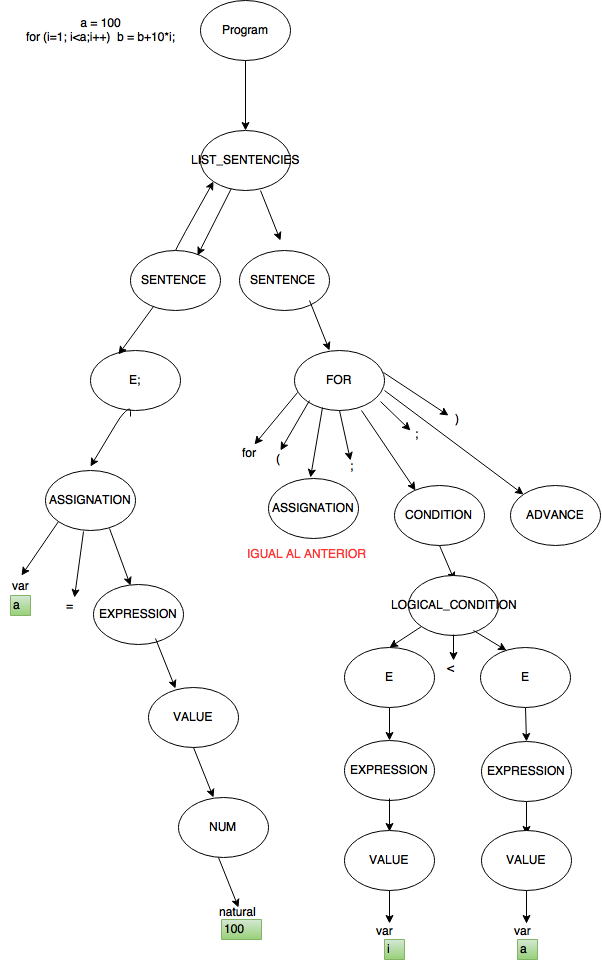
\includegraphics[scale=0.7]{imgs/ejemploGramatica.png}
\end{center}

\section{Descripción}

Asumimos que ASIGNACION $\rightarrow$ VAR = NUM 

Asumimos que los Registers toman únicamente literales de tipos básicos.

Decidimos que los comentarios se reescriben en la línea de abajo para mayor claridad del código.

El único newline que nos interesa es entre \{ ; \{ \} ) \} y \#

Gramática de atributos:

\begin{itemize}
\item \textbf{Value:} string (\textit{sintetizado}) es el código de salida del parser arreglado.
\item \textbf{Level:} int (\textit{heredado}) almacena el nivel de indentación de la producción actual.
\item \textbf{Type:} string (\textit{sintetizado}) representa el tipo de la expresión en cuestión.
\end{itemize}

\section{Compilación y ejecución}

\section{Casos de prueba}

\section{Resultados}

\section{Conclusión}

\section{Referencias}

\end{document}
